%%%%%%%%%%%%%%%%%%%%%%%%%%%%%%%%%%%%%%%%%%%%%%%%%%%%%%%%%%%%%%%%%%%%%%%%%%%%%%%%%%%%%%%
\cleardoublepage
\thispagestyle{empty}
\begin{center}
\vspace*{3cm}
{\huge \bf Part I}\\ \vspace*{1cm}
{\Huge \bf Title of this Part}\\\vspace*{0.2cm}
{\Huge \bf Being Longer than One Line}\\\vspace*{3cm}
\begin{figure}[ht]
\centering
\includegraphics[height=6cm]{figures/part1_notesAndWaveform_orange}
\end{figure}
\end{center}
\addcontentsline{toc}{part}{I\hspace {1em}Title of this Part Being Longer than One Line}
\label{par:part1}
\newpage
\quad
\thispagestyle{empty}
\newpage

%%%%%%%%%%%%%%%%%%%%%%%%%%%%%%%%%%%%%%%%%%%%%%%%%%%%%%%%%%%%%%%%%%%%%%%%%%%%%%%%%%%%%%%


%%%%%%%%%%%%%%%%%%%%%%%%%%%%%%%%%%%%%%%%%%%%%%%%%%%%%%%%%%%%%%%%%%%%%%%%%%%%%%%%%%%%%%%
\chapter{Theoretic Foundations}
\label{chapter:Foundations}
%%%%%%%%%%%%%%%%%%%%%%%%%%%%%%%%%%%%%%%%%%%%%%%%%%%%%%%%%%%%%%%%%%%%%%%%%%%%%%%%%%%%%%%

Each chapter should start with a small summary discussing the content and the relation
of the sections. In this chapter, we elaborate on the theoretical background, 
foundations and concepts that are being used in the thesis. In particular, we 
focus on latex construct that are typically used in thesis documents.

When using labels, please avoid collisions in the label names.


%%%%%%%%%%%%%%%%%%%%%%%%%%%%%%%%%%%%%%%%%%%%%%%%%%%%%%%%%%%%%%%%%%%%%%%%%%%%%%%%%%%%%%%
\section{Ordinary Differential Equations}
\label{section:ode}
%%%%%%%%%%%%%%%%%%%%%%%%%%%%%%%%%%%%%%%%%%%%%%%%%%%%%%%%%%%%%%%%%%%%%%%%%%%%%%%%%%%%%%%

An \ac{ODE} is an equation of the form
\begin{equation}
  \frac{\mathrm{d} y}{\mathrm{d} t} = f(t, y),
  \label{eq:general_ode}
\end{equation}
where $y$ is the \emph{unknown function}, $t$ is the \emph{independent variable}, and $f(t, y)$ is a function of both, $t$ and $y$. Implicitly, $y$ is dependent on $t$, i.\ e., $y = y(t)$. In the scope of this work, $t$ denotes time. The term \emph{ordinary} means that $y$ is a function of a single variable and, thus, an "ordinary" derivative is used, i.\ e., $\frac{\mathrm{d} y}{\mathrm{d} t}$ \cite{Gockenbach2011}.

To \emph{solve} an \ac{ODE} means to find a function $y$ that satisfies \Equation{eq:general_ode}. Such $y$ is called a \emph{solution}.

\acp{ODE} are used to model dynamical systems \cite{Karlsson2019}. An example of a dynamical system that can be described by an \ac{ODE} is an electrical circuit containing capacitive elements, such as a diode clipper circuit \cite{Yeh2007}. % TODO: Reference a section on the diode clipper
Since an equation of the form \Equation{eq:general_ode} describes a rate of change $\frac{\mathrm{d} y}{\mathrm{d} t}$, its solution will not be a single function, but rather a family of functions or a parametrized function. To obtain a unique solution, we need to specify an \emph{\ac{IC}}. An \ac{ODE} together with an initial condition makes up an \emph{\ac{IVP}}.

Some classes of \acp{IVP} can be solved analytically. However, for the most interesting applications, e.\ g., in the domain of analog audio effects, the corresponding \acp{IVP} are solved using numerical methods, i.\ e., specialized algorithms using discrete points to approximate the true solution \cite{Gockenbach2011}. 

A group of numerical methods is called \emph{time-stepping methods}. Given a grid of time instants $t_0 < t_1 < \dots < t_n$ and a value of $y$ at $t_0$, $y(t_0$) these methods use the following identity
\begin{equation}
  y(t_{i+1}) = y(t_{i}) + \int \limits_{t_i}^{t_{i+1}} f(s, y(s)) \mathrm{d} s
  \label{eq:time_stepping_identity}
\end{equation}
to approximate the value $y$ at the points on the grid, $y(t_1), y(t_2), \dots, y(t_n)$. The core idea is to approximate the integral in \Equation{eq:time_stepping_identity}. Thus, the process of solving an \ac{IVP} is often referred to as \emph{integrating} the \ac{ODE} \cite{Gockenbach2011}.

%%%%%%%%%%%%%%%%%%%%%%%%%%%%%%%%%%%%%%%%%%%%%%%%%%%%%%%%%%%%%%%%%%%%%%%%%%%%%%%%%%%%%%%
\section{Deep Learning}
\label{section:deep_learning}
%%%%%%%%%%%%%%%%%%%%%%%%%%%%%%%%%%%%%%%%%%%%%%%%%%%%%%%%%%%%%%%%%%%%%%%%%%%%%%%%%%%%%%%

Broadly speaking, machine learning is a field of engineering using data to improve on a task at hand \cite{Goodfellow-et-al-2016}. A subfield of machine learning called deep learning uses \acp{ANN} for the improvement process. 

An \ac{ANN} is a model whose goal is to approximate some function $f^*$ \cite{Goodfellow-et-al-2016}. A \emph{feedforward network} or an \ac{MLP} is an input-to-output mapping. For example, in the context of audio signal processing, $f^*$ could be a mapping of an input signal $s_{in}(t)$ to an output signal $s_{out}(t)$, i.\ e., $s_{out}(t) = f*(s_{in}(t))$. The mapping $f$ defined by an \ac{MLP}, $\hat{s}_{out}(t) = f(s_{in}(t); \pmb{\theta})$, is dependent on the parameter vector $\pmb{\theta}$. The learning process aims at finding a parameter vector $\pmb{\theta^*}$ that allows for a sufficiently accurate approximation of $f^*$ by $f$.

% TODO: Add figure with a MLP

A feedforward network consists of \emph{layers} which define the subsequent stages of computations. The first layer is called the \emph{input layer} and the last layer is called the \emph{output layer}. The layers in between are called the \emph{hidden layers}, because we do not observe their output directly. Each layer consists of a set of \emph{units}: affine transformations of unit's inputs followed by a nonlinearity. Each unit in a layer receives outputs of all units in the previous layer at its input and outputs a single scalar. The number of layers determines the \emph{depth} of the model. Feedforward networks with at least 1 hidden layer are called \emph{deep}. The number of units in a layer determines its \emph{width}.

\acp{MLP} are \emph{universal function approximators}, i.\ e., they can approximate an arbitrary function (fulfilling very mild criteria) with an arbitrarily small error given enough width or depth \cite{Goodfellow-et-al-2016}.

%%%%%%%%%%%%%%%%%%%%%%%%%%%%%%%%%%%%%%%%%%%%%%%%%%%%%%%%%%%%%%%%%%%%%%%%%%%%%%%%%%%%%%%
\section*{Training of Neural Networks}
%%%%%%%%%%%%%%%%%%%%%%%%%%%%%%%%%%%%%%%%%%%%%%%%%%%%%%%%%%%%%%%%%%%%%%%%%%%%%%%%%%%%%%%

Training of \acp{ANN} is done using an algorithm from the \emph{gradient descent} family of algorithms \cite{Goodfellow-et-al-2016}. In general, gradient descent methodology requires specifying a \emph{loss} or a \emph{target function} between the network's output and the desired output. The optimization then proceeds by sampling a \emph{minibatch} of examples from the \emph{training set} in each iteration, processing them with the network, and calculating the loss. Afterwards, the gradient of the loss with respect to the parameters is computed and \emph{backpropagated} through the network using the chain rule of derivatives. After calculating the gradient of the loss with respect to each individual parameter, a step in the direction of the negated gradient is performed (steepest descent). The size of the step is determined by the \emph{learning rate}. Some algorithms use a different step size for each parameter, for example, Adam \cite{Kingma2017}.

%%%%%%%%%%%%%%%%%%%%%%%%%%%%%%%%%%%%%%%%%%%%%%%%%%%%%%%%%%%%%%%%%%%%%%%%%%%%%%%%%%%%%%%
\section*{Architectures}
%%%%%%%%%%%%%%%%%%%%%%%%%%%%%%%%%%%%%%%%%%%%%%%%%%%%%%%%%%%%%%%%%%%%%%%%%%%%%%%%%%%%%%%

As deep learning is a widely and actively pursued field of science, there exist many different neural network architectures beyond the \ac{MLP}. They are often designed for the task at hand using expert knowledge or heuristics \cite{Goodfellow-et-al-2016}. In this section, two highly successful architectures are presented, both of them relevant for this thesis.

%%%%%%%%%%%%%%%%%%%%%%%%%%%%%%%%%%%%%%%%%%%%%%%%%%%%%%%%%%%%%%%%%%%%%%%%%%%%%%%%%%%%%%%
\subsection*{Long Short-Term Memory}
%%%%%%%%%%%%%%%%%%%%%%%%%%%%%%%%%%%%%%%%%%%%%%%%%%%%%%%%%%%%%%%%%%%%%%%%%%%%%%%%%%%%%%%

\Ac{RNN} is a neural network that maintains a \emph{feedback} connection, i.\ e., a connection from its output to its input. Typically, to calculate the current output, the previous output is taken as part of the input. This step-by-step processing is characteristic to sequence modeling, where \acp{RNN} are found most useful.

% TODO: Add figure with an LSTM

A particularly successful \ac{RNN} architecture is the \ac{LSTM} \cite{Hochreiter1997}. \ac{LSTM} uses \emph{gating units} to allow or disallow its \emph{memory cells} to be updated during processing. This helps to learn long-term dependencies which are crucial for the network to maintain a notion of a context.

\ac{LSTM} has been successfully applied to guitar amplifier \cite{Wright2019,Wrightetal2020} and time-varying effects modeling \cite{Wright2020}.

%%%%%%%%%%%%%%%%%%%%%%%%%%%%%%%%%%%%%%%%%%%%%%%%%%%%%%%%%%%%%%%%%%%%%%%%%%%%%%%%%%%%%%%
\subsection*{Residual Networks}
%%%%%%%%%%%%%%%%%%%%%%%%%%%%%%%%%%%%%%%%%%%%%%%%%%%%%%%%%%%%%%%%%%%%%%%%%%%%%%%%%%%%%%%

% TODO: Add figure with a ResNet
Another architecture significant to this work is the \ac{ResNet} \cite{He2015}. Its characteristic feature is the so-called \emph{\ac{ResBlock}} containing a \emph{skip connection}. The skip connection provides a direct path from the input to the output which allows for summing the input with the network's output. It effectively makes the network learn not the mapping $f^*(\pmb{x})$ but the residual $h^*(\pmb{x}) = f^*(\pmb{x}) - \pmb{x}$. On the one hand, it alleviates the problem of the \emph{vanishing gradient} \cite{Goodfellow-et-al-2016} and eventually allows for training very deep architectures with hundreds of layers \cite{He2015}. Depth is one of the most significant factors in neural network design, thus, being able to train deeper and deeper architectures allows for improving performance on the desired tasks. On the other hand, the skip connection can simplify the training process; instead of learning a complete function, the network must only learn its residual. For example, if the true mapping is the identity function, it is easier to learn the residual (which is $0$ everywhere) rather than the identity itself, which would involve approximating a hyperplane with nonlinear units \cite{He2015}.

%%%%%%%%%%%%%%%%%%%%%%%%%%%%%%%%%%%%%%%%%%%%%%%%%%%%%%%%%%%%%%%%%%%%%%%%%%%%%%%%%%%%%%%
\subsection{Neural Ordinary Differential Equations}
\label{sec:neural_odes}
%%%%%%%%%%%%%%%%%%%%%%%%%%%%%%%%%%%%%%%%%%%%%%%%%%%%%%%%%%%%%%%%%%%%%%%%%%%%%%%%%%%%%%%

%TODO: Add citations
%TODO: Add ODENet figure

It has been observed that learning the residual instead of the function can be viewed as an Euler step of solving a differential equation. In the Euler method of solving \acp{ODE}, function's value at time step $t_i$ is approximated by adding the value of the derivative at time step $t_{i-1}$ multiplied by the time step size $t_i - t_{i-1}$ to the function's value at $t_i$. \cite{Chen2018} stated this observation explicitly and proposed to change the discrete scheme to a continuous one. In such a scheme, the network learns not the residual but the derivative of the desired function. This "derivative network" is supplied to a numerical solver of choice. The loss is calculated using the solver's (not the network's) output. Such generically defined architecture was named ODENet. The backpropagation through the solver's operations can be done in constant time using the adjoint sensitivity method \cite{Chen2018}.

\cite{Karlsson2019} successfully applied ODENet to model dynamical systems, i.\ e., systems governed by \acp{ODE}. 

%%%%%%%%%%%%%%%%%%%%%%%%%%%%%%%%%%%%%%%%%%%%%%%%%%%%%%%%%%%%%%%%%%%%%%%%%%%%%%%%%%%%%%%
\section{Virtual Analog Modeling}
\label{sec:virtual_analog_modeling}
%%%%%%%%%%%%%%%%%%%%%%%%%%%%%%%%%%%%%%%%%%%%%%%%%%%%%%%%%%%%%%%%%%%%%%%%%%%%%%%%%%%%%%%
\Ac{VA} effects are digital emulations of audio systems that were originally built using analog electronic or electromechanical components \cite{Zoelzer2011}. They arose out of the demand for the reproduction of characteristic tonal distortions of these devices but with the digital stability and the ease of integration with existing software. Devices modelled range from filters, to time-varying effects, amplifiers, mechanical reverb units, and tape or vinyl distortions.

One can distinguish three general approaches to \ac{VA} modeling \cite{Kiiski2016,Wright2020}. In \emph{black-box} modelling, only the input-output relation of a system is examined and a signal model is constructed to mimic that behavior. Neural networks have successfully been applied to this kind of modeling for guitar amplifiers \cite{Wright2019,Wrightetal2020}. In \emph{white-box} modelling an internal structure of the system under study is examined and used to construct an algorithm aiming at reproducing its behavior. Sometimes it is referred to as \emph{physical modeling}. Typical approaches in this category are a numerical solution of \acp{ODE} derived from electronic circuit analysis \cite{Yeh2007,Eichas2014} or wave-digital filters \cite{PASPWEB2010}. \emph{Grey-box} modeling falls somewhere in between the two already mentioned approaches, where we use some knowledge about the inner workings of the device under study to design a model and, subsequently, take advantage of the input and output data to adjust the model's parameters. This approach has been successfully applied to time-varying effects modeling, like a phaser or a flanger \cite{Kiiski2016,Wright2020}, where a \ac{LFO} signal is estimated and used for conditioning the model.


%%%%%%%%%%%%%%%%%%%%%%%%%%%%%%%%%%%%%%%%%%%%%%%%%%%%%%%%%%%%%%%%%%%%%%%%%%%%%%%%%%%%%%%
\section{Modeled Systems}
\label{sec:modeled_systems}
%%%%%%%%%%%%%%%%%%%%%%%%%%%%%%%%%%%%%%%%%%%%%%%%%%%%%%%%%%%%%%%%%%%%%%%%%%%%%%%%%%%%%%%
The aim of this work is to investigate the applicability of the ODENet architecture to \ac{VA} modeling of audio effects. The main goal is to model a phaser pedal. However, in order to get intuition behind this type of architecture, a simpler, time-invariant system was modeled, namely, a first-order diode clipper. This section describes both these devices.

%%%%%%%%%%%%%%%%%%%%%%%%%%%%%%%%%%%%%%%%%%%%%%%%%%%%%%%%%%%%%%%%%%%%%%%%%%%%%%%%%%%%%%%
\subsection{Diode Clipper}
\label{subsec:diode_clipper_intro}
%%%%%%%%%%%%%%%%%%%%%%%%%%%%%%%%%%%%%%%%%%%%%%%%%%%%%%%%%%%%%%%%%%%%%%%%%%%%%%%%%%%%%%%
\begin{figure}
  \centering
  %%%%%%%%%%%%%%%%%%%%%%%%%%%%%%%%%%%%%%%%%%%%%%%%%%%%%%%%%%%%%%%%%%%%%%%%%%%%%%%%%%%%%%%
\section{Diode Clipper Circuit}
\label{subsec:diode_clipper_intro}
%%%%%%%%%%%%%%%%%%%%%%%%%%%%%%%%%%%%%%%%%%%%%%%%%%%%%%%%%%%%%%%%%%%%%%%%%%%%%%%%%%%%%%%
\begin{figure}
  \centering
  %%%%%%%%%%%%%%%%%%%%%%%%%%%%%%%%%%%%%%%%%%%%%%%%%%%%%%%%%%%%%%%%%%%%%%%%%%%%%%%%%%%%%%%
\section{Diode Clipper Circuit}
\label{subsec:diode_clipper_intro}
%%%%%%%%%%%%%%%%%%%%%%%%%%%%%%%%%%%%%%%%%%%%%%%%%%%%%%%%%%%%%%%%%%%%%%%%%%%%%%%%%%%%%%%
\begin{figure}
  \centering
  %%%%%%%%%%%%%%%%%%%%%%%%%%%%%%%%%%%%%%%%%%%%%%%%%%%%%%%%%%%%%%%%%%%%%%%%%%%%%%%%%%%%%%%
\section{Diode Clipper Circuit}
\label{subsec:diode_clipper_intro}
%%%%%%%%%%%%%%%%%%%%%%%%%%%%%%%%%%%%%%%%%%%%%%%%%%%%%%%%%%%%%%%%%%%%%%%%%%%%%%%%%%%%%%%
\begin{figure}
  \centering
  \input{figures/tikz/diode_clipper.tex}
  \caption{Diode clipper circuit.}
  \label{fig:diode_clipper_circuit}
\end{figure}

The first-order diode clipper is a circuit frequently used to achieve signal distortion, e.g., in guitar amplifiers. Its schematic is shown in \Figure{fig:diode_clipper_circuit}. It can be regarded as consisting of two parts: an RC lowpass filter and a diode limiter.

Voltages and currents in this section are dependent on time, i.e., $V = V(t), I= I(t)$. For readability, this dependence is not stated explicitly in the equations.

%%%%%%%%%%%%%%%%%%%%%%%%%%%%%%%%%%%%%%%%%%%%%%%%%%%%%%%%%%%%%%%%%%%%%%%%%%%%%%%%%%%%%%%
\subsection{RC Lowpass Filter}
%%%%%%%%%%%%%%%%%%%%%%%%%%%%%%%%%%%%%%%%%%%%%%%%%%%%%%%%%%%%%%%%%%%%%%%%%%%%%%%%%%%%%%%

\begin{figure}
  \centering
  \input{figures/tikz/rc_lowpass.tex}
  \caption{RC lowpass filter.}
  \label{fig:rc_lowpass}
\end{figure}

The first part of the diode clipper circuit is an RC lowpass filter. An RC lowpass filter is shown in \Figure{fig:rc_lowpass}. Given that the input voltage $V_\text{in}$ is a sine wave at frequency $f$, the input-output voltage relation is governed by the following equation
\begin{equation}
  V_\text{out} = \frac{X_C}{\sqrt{R^2 + X_C^2}} V_\text{in},
  \label{eq:rc_circuit}
\end{equation}
where $V_\text{out}$ is the output voltage, $X_C=\frac{1}{2\pi f C}$ is the capacitive reactance of the capacitor in the circuit, $C$ is its capacitance, and $R$ is the resistor's resistance.

The capacitor impedes low frequencies more; the lower the frequency, the higher the capacitive reactance. More capacitive reactance means larger voltage drop on the capacitor. Thus, assuming a constant magnitude across all frequencies of the input voltage, the output voltage is higher for low frequencies. Therefore, the circuit behaves like a lowpass filter.

Considering an arbitrary input waveform, we may derive a differential equation that describes the circuit \cite{Horowitz2015}. The current $I$ through the capacitor is proportional to the rate of change of the voltage across it

\begin{equation}
  I = C \frac{\mathrm{d}V_\text{out}}{\mathrm{d} t}.
  \label{eq:current_through_capacitor}
\end{equation}

The current flowing through the resistor can be calculated using the Ohm's law as a ratio of the voltage drop across the resistor to its resistance

\begin{equation}
  I = \frac{V_\text{in} - V_\text{out}}{R}.
  \label{eq:current_through_resistor}
\end{equation}

Because the same current flows through the resistor and the capacitor we can equate the right-hand sides of \Equation{eq:current_through_capacitor} and \Equation{eq:current_through_resistor}. After dividing by $C$, we obtain the final form of the \ac{ODE} describing the RC circuit

\begin{equation}
  \frac{\mathrm{d}V_\text{out}}{\mathrm{d} t} = \frac{V_\text{in} - V_\text{out}}{RC}.
\end{equation}



%%%%%%%%%%%%%%%%%%%%%%%%%%%%%%%%%%%%%%%%%%%%%%%%%%%%%%%%%%%%%%%%%%%%%%%%%%%%%%%%%%%%%%%
\subsection{Diode Limiter}
%%%%%%%%%%%%%%%%%%%%%%%%%%%%%%%%%%%%%%%%%%%%%%%%%%%%%%%%%%%%%%%%%%%%%%%%%%%%%%%%%%%%%%%
\begin{figure}
  \centering
  \input{figures/tikz/diode_limiter.tex}
  \caption{Diode limiter circuit.}
  \label{fig:diode_limiter}
\end{figure}

The second part of the diode clipper is the diode limiter also called a \emph{diode clamp} \cite{Malvino2016}. Its circuit is shown in \Figure{fig:diode_limiter}. It consists of two inversely polarized diodes and a resistor. This circuit could be further divided into a \emph{positive clipper} (by removing the diode on the left) and a \emph{negative clipper} (by removing the diode on the right). These names refer to which part of the input \ac{AC} signal (the positive or the negative) is removed at the output.

If the diodes were ideal, i.e., they would behave as an open for voltages across smaller than 0 and as a short for voltages across larger than 0, $V_\text{out}$ would always be 0. However, to a second approximation, the diodes cause a voltage drop of \SI{0.7}{V} when conducting. Thus, the voltage cannot exceed the \SIrange{-0.7}{0.7}{V} range, being clamped when attempting to do so. The positive clipper guards the upper limit and the negative clipper guards the lower limit. The effect of passing an \ac{AC} signal through the diode limiter is shown in \Figure{fig:diode_limiter_signal}.

\cite{Yeh2007} contains a small-signal interpretation of the diode limiter circuit.

\begin{figure}
  \centering
  \input{figures/tikz/diode_limiter_signal.tex}
  \caption{Impact of the diode limiter on the input sinusoidal voltage. Values that exceed the \SIrange{-0.7}{0.7}{V} range are clamped and the signal is distorted.}
  \label{fig:diode_limiter_signal}
\end{figure}


%%%%%%%%%%%%%%%%%%%%%%%%%%%%%%%%%%%%%%%%%%%%%%%%%%%%%%%%%%%%%%%%%%%%%%%%%%%%%%%%%%%%%%%
\subsection{First-Order Diode Clipper}
%%%%%%%%%%%%%%%%%%%%%%%%%%%%%%%%%%%%%%%%%%%%%%%%%%%%%%%%%%%%%%%%%%%%%%%%%%%%%%%%%%%%%%%
Combining the RC lowpass filter (\Figure{fig:rc_lowpass}) and the diode limiter (\Figure{fig:diode_limiter}) yields the first-order diode clipper (\Figure{fig:diode_clipper_circuit}). It is called "first-order" because only a single capacitor is used \cite{Parker2019}. If the input voltage is within the limiter's operational range, the circuit acts as a lowpass filter. If the voltage exceeds this range, it is clipped at the output and distortion is introduced.

The first-order diode clipper can be described by a nonlinear \ac{ODE} \cite{Yeh2007}
\begin{equation}
  \frac{\mathrm{d} V_\text{out}}{\mathrm{d}t} = \frac{V_\text{in} - V_\text{out}}{RC} - 2 \frac{I_\text{s}}{C} \sinh \left(\frac{V_\text{out}}{V_\text{t}}\right),
  \label{eq:diode_clipper_equation}
\end{equation}
where $V_\text{in}$ is the input voltage, $V_\text{out}$ is the output voltage, $t$ denotes time, $R$ is the serial resistance, $C$ is the parallel capacity, $I_\text{s}$ is the reverse saturation current, and $V_\text{t}$ is the thermal voltage. The last two are parameters of the diodes that can be measured \cite{Yeh2007}.

The parameter values of discrete elements used in the experiments were taken from \cite{Yeh2008}. They are summarized in \Table{tab:diode_clipper_element_parameters}.

\begin{table}
  \centering
  \caption{Parameter values of the discrete elements used in the diode clipper circuit. Source: \cite{Yeh2008}.}
  \begin{tabular}{c|c}
    \toprule
    \textbf{Parameter} & \textbf{Value} \\
    \midrule
    $R$ & \SI{2.2}{k\ohm} \\
    $C$ & \SI{10}{nF} \\
    $I_\text{s}$ & \SI{2.52}{nA} \\
    $V_\text{t}$ & \SI{45.3}{mV} \\
    \hline
  \end{tabular}
  \label{tab:diode_clipper_element_parameters}
\end{table}

$V_\text{in}$ is typically on the order of volts.

%%%%%%%%%%%%%%%%%%%%%%%%%%%%%%%%%%%%%%%%%%%%%%%%%%%%%%%%%%%%%%%%%%%%%%%%%%%%%%%%%%%%%%%
\subsection{Relation to Other Work}
%%%%%%%%%%%%%%%%%%%%%%%%%%%%%%%%%%%%%%%%%%%%%%%%%%%%%%%%%%%%%%%%%%%%%%%%%%%%%%%%%%%%%%%

The first-order diode clipper is a system particularly interesting in the context of ODENet, because it is governed by a known \ac{ODE} \cite{Yeh2007,Yeh2008}. Additionally, it was already modeled using a \ac{ResNet}-like architecture in \cite{Parker2019}. Thus, learning to imitate the diode clipper allowed the validation of ODENet and comparison to 
\begin{itemize}
    \item an \ac{LSTM}-based architecture from \cite{Wrightetal2020},
    \item a \ac{ResNet}-like architecture from \cite{Parker2019}, and
    \item a numerical solution using the \ac{ODE} from \cite{Yeh2007,Yeh2008}.
\end{itemize}

  \caption{Diode clipper circuit.}
  \label{fig:diode_clipper_circuit}
\end{figure}

The first-order diode clipper is a circuit frequently used to achieve signal distortion, e.g., in guitar amplifiers. Its schematic is shown in \Figure{fig:diode_clipper_circuit}. It can be regarded as consisting of two parts: an RC lowpass filter and a diode limiter.

Voltages and currents in this section are dependent on time, i.e., $V = V(t), I= I(t)$. For readability, this dependence is not stated explicitly in the equations.

%%%%%%%%%%%%%%%%%%%%%%%%%%%%%%%%%%%%%%%%%%%%%%%%%%%%%%%%%%%%%%%%%%%%%%%%%%%%%%%%%%%%%%%
\subsection{RC Lowpass Filter}
%%%%%%%%%%%%%%%%%%%%%%%%%%%%%%%%%%%%%%%%%%%%%%%%%%%%%%%%%%%%%%%%%%%%%%%%%%%%%%%%%%%%%%%

\begin{figure}
  \centering
  \begin{tikzpicture}
%--------start graphics code --------
% \draw[step=0.5,very thin, black!20] (-1,-0.5) grid (6,2.5);
\path (0,0) coordinate (ref_gnd);
\draw
  (ref_gnd)++(0,2) node[ocirc] {}
  node[xshift=-2mm,yshift=4mm] {$V_{in}$}
  to [R=\(R\)] ++(2,0) node[circ] {}
  to ++(1,0)  node[ocirc] {}
  node[yshift=4mm] {$V_{out}$}
  ++(-1,0)
  to [C=\(C\)] ++(0,-2)
  node[ground] {};
%--------end graphics code ----------
\end{tikzpicture}

  \caption{RC lowpass filter.}
  \label{fig:rc_lowpass}
\end{figure}

The first part of the diode clipper circuit is an RC lowpass filter. An RC lowpass filter is shown in \Figure{fig:rc_lowpass}. Given that the input voltage $V_\text{in}$ is a sine wave at frequency $f$, the input-output voltage relation is governed by the following equation
\begin{equation}
  V_\text{out} = \frac{X_C}{\sqrt{R^2 + X_C^2}} V_\text{in},
  \label{eq:rc_circuit}
\end{equation}
where $V_\text{out}$ is the output voltage, $X_C=\frac{1}{2\pi f C}$ is the capacitive reactance of the capacitor in the circuit, $C$ is its capacitance, and $R$ is the resistor's resistance.

The capacitor impedes low frequencies more; the lower the frequency, the higher the capacitive reactance. More capacitive reactance means larger voltage drop on the capacitor. Thus, assuming a constant magnitude across all frequencies of the input voltage, the output voltage is higher for low frequencies. Therefore, the circuit behaves like a lowpass filter.

Considering an arbitrary input waveform, we may derive a differential equation that describes the circuit \cite{Horowitz2015}. The current $I$ through the capacitor is proportional to the rate of change of the voltage across it

\begin{equation}
  I = C \frac{\mathrm{d}V_\text{out}}{\mathrm{d} t}.
  \label{eq:current_through_capacitor}
\end{equation}

The current flowing through the resistor can be calculated using the Ohm's law as a ratio of the voltage drop across the resistor to its resistance

\begin{equation}
  I = \frac{V_\text{in} - V_\text{out}}{R}.
  \label{eq:current_through_resistor}
\end{equation}

Because the same current flows through the resistor and the capacitor we can equate the right-hand sides of \Equation{eq:current_through_capacitor} and \Equation{eq:current_through_resistor}. After dividing by $C$, we obtain the final form of the \ac{ODE} describing the RC circuit

\begin{equation}
  \frac{\mathrm{d}V_\text{out}}{\mathrm{d} t} = \frac{V_\text{in} - V_\text{out}}{RC}.
\end{equation}



%%%%%%%%%%%%%%%%%%%%%%%%%%%%%%%%%%%%%%%%%%%%%%%%%%%%%%%%%%%%%%%%%%%%%%%%%%%%%%%%%%%%%%%
\subsection{Diode Limiter}
%%%%%%%%%%%%%%%%%%%%%%%%%%%%%%%%%%%%%%%%%%%%%%%%%%%%%%%%%%%%%%%%%%%%%%%%%%%%%%%%%%%%%%%
\begin{figure}
  \centering
  \begin{tikzpicture}
%--------start graphics code --------
% \draw[step=0.5,very thin, black!20] (-1,-0.5) grid (6,2.5);
\path (0,0) coordinate (ref_gnd);
\draw
  (ref_gnd)++(0,2) node[ocirc] {}
  node[xshift=-2mm,yshift=4mm] {$V_{in}$}
  to [R=\(R\)] ++(2,0) node[circ] {}
  to ++(2,0)  node[circ] {}
  to ++(1,0)  node[ocirc] {} {}
  node[yshift=4mm] {$V_{out}$}
  ++(-1,0)
  to [D] ++(0,-2)
  to ++(-1,0)
  node[ground] {}
  to ++(-1,0)
  to [D] ++(0,2);
%--------end graphics code ----------
\end{tikzpicture}

  \caption{Diode limiter circuit.}
  \label{fig:diode_limiter}
\end{figure}

The second part of the diode clipper is the diode limiter also called a \emph{diode clamp} \cite{Malvino2016}. Its circuit is shown in \Figure{fig:diode_limiter}. It consists of two inversely polarized diodes and a resistor. This circuit could be further divided into a \emph{positive clipper} (by removing the diode on the left) and a \emph{negative clipper} (by removing the diode on the right). These names refer to which part of the input \ac{AC} signal (the positive or the negative) is removed at the output.

If the diodes were ideal, i.e., they would behave as an open for voltages across smaller than 0 and as a short for voltages across larger than 0, $V_\text{out}$ would always be 0. However, to a second approximation, the diodes cause a voltage drop of \SI{0.7}{V} when conducting. Thus, the voltage cannot exceed the \SIrange{-0.7}{0.7}{V} range, being clamped when attempting to do so. The positive clipper guards the upper limit and the negative clipper guards the lower limit. The effect of passing an \ac{AC} signal through the diode limiter is shown in \Figure{fig:diode_limiter_signal}.

\cite{Yeh2007} contains a small-signal interpretation of the diode limiter circuit.

\begin{figure}
  \centering
  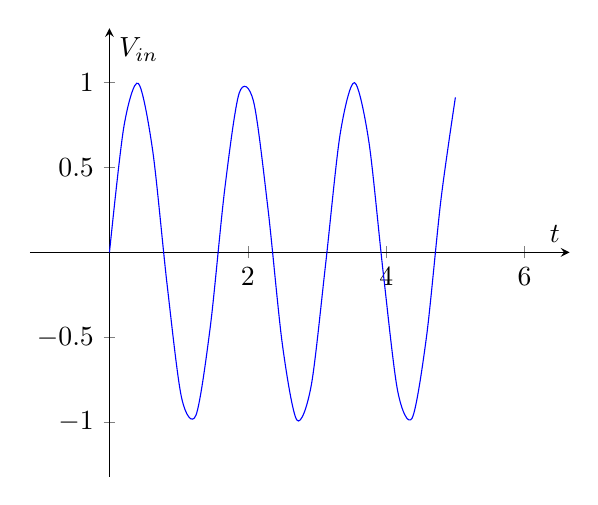
\begin{tikzpicture}
    \begin{axis}[
        domain=0:5,
        axis lines = middle,
        xmin = -0.5,
        xmax = 6,
        ymin = -1.1,
        ymax = 1.1,
        xlabel = $t$,
        ylabel = $V_{in}$,
        enlargelimits = true,
    ]
        \addplot[smooth,mark=none,color=blue] {sin(4*deg(x))};
    \end{axis}
\end{tikzpicture}
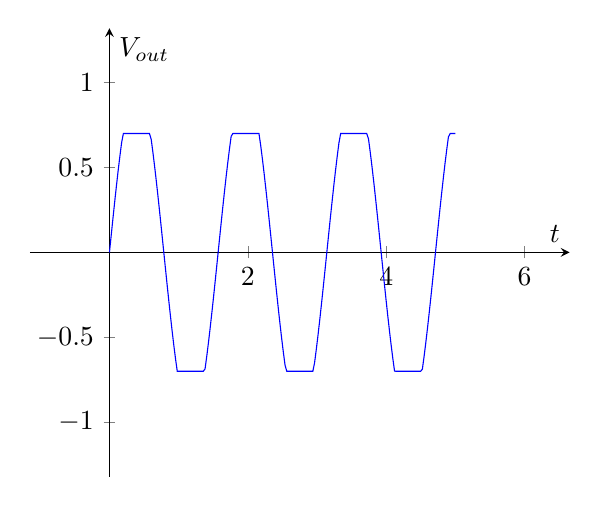
\begin{tikzpicture}
    \begin{axis}[
        domain=0:5,
        axis lines = middle,
        xmin = -0.5,
        xmax = 6,
        ymin = -1.1,
        ymax = 1.1,
        xlabel = $t$,
        ylabel = $V_{out}$,
        enlargelimits = true,
        y filter/.expression={y > 0.7 ? 0.7 : (y < -0.7 ? -0.7 : y)},
    ]
        \addplot[samples=200,mark=none,color=blue] {sin(4*deg(x))};
    \end{axis}
\end{tikzpicture}

  \caption{Impact of the diode limiter on the input sinusoidal voltage. Values that exceed the \SIrange{-0.7}{0.7}{V} range are clamped and the signal is distorted.}
  \label{fig:diode_limiter_signal}
\end{figure}


%%%%%%%%%%%%%%%%%%%%%%%%%%%%%%%%%%%%%%%%%%%%%%%%%%%%%%%%%%%%%%%%%%%%%%%%%%%%%%%%%%%%%%%
\subsection{First-Order Diode Clipper}
%%%%%%%%%%%%%%%%%%%%%%%%%%%%%%%%%%%%%%%%%%%%%%%%%%%%%%%%%%%%%%%%%%%%%%%%%%%%%%%%%%%%%%%
Combining the RC lowpass filter (\Figure{fig:rc_lowpass}) and the diode limiter (\Figure{fig:diode_limiter}) yields the first-order diode clipper (\Figure{fig:diode_clipper_circuit}). It is called "first-order" because only a single capacitor is used \cite{Parker2019}. If the input voltage is within the limiter's operational range, the circuit acts as a lowpass filter. If the voltage exceeds this range, it is clipped at the output and distortion is introduced.

The first-order diode clipper can be described by a nonlinear \ac{ODE} \cite{Yeh2007}
\begin{equation}
  \frac{\mathrm{d} V_\text{out}}{\mathrm{d}t} = \frac{V_\text{in} - V_\text{out}}{RC} - 2 \frac{I_\text{s}}{C} \sinh \left(\frac{V_\text{out}}{V_\text{t}}\right),
  \label{eq:diode_clipper_equation}
\end{equation}
where $V_\text{in}$ is the input voltage, $V_\text{out}$ is the output voltage, $t$ denotes time, $R$ is the serial resistance, $C$ is the parallel capacity, $I_\text{s}$ is the reverse saturation current, and $V_\text{t}$ is the thermal voltage. The last two are parameters of the diodes that can be measured \cite{Yeh2007}.

The parameter values of discrete elements used in the experiments were taken from \cite{Yeh2008}. They are summarized in \Table{tab:diode_clipper_element_parameters}.

\begin{table}
  \centering
  \caption{Parameter values of the discrete elements used in the diode clipper circuit. Source: \cite{Yeh2008}.}
  \begin{tabular}{c|c}
    \toprule
    \textbf{Parameter} & \textbf{Value} \\
    \midrule
    $R$ & \SI{2.2}{k\ohm} \\
    $C$ & \SI{10}{nF} \\
    $I_\text{s}$ & \SI{2.52}{nA} \\
    $V_\text{t}$ & \SI{45.3}{mV} \\
    \hline
  \end{tabular}
  \label{tab:diode_clipper_element_parameters}
\end{table}

$V_\text{in}$ is typically on the order of volts.

%%%%%%%%%%%%%%%%%%%%%%%%%%%%%%%%%%%%%%%%%%%%%%%%%%%%%%%%%%%%%%%%%%%%%%%%%%%%%%%%%%%%%%%
\subsection{Relation to Other Work}
%%%%%%%%%%%%%%%%%%%%%%%%%%%%%%%%%%%%%%%%%%%%%%%%%%%%%%%%%%%%%%%%%%%%%%%%%%%%%%%%%%%%%%%

The first-order diode clipper is a system particularly interesting in the context of ODENet, because it is governed by a known \ac{ODE} \cite{Yeh2007,Yeh2008}. Additionally, it was already modeled using a \ac{ResNet}-like architecture in \cite{Parker2019}. Thus, learning to imitate the diode clipper allowed the validation of ODENet and comparison to 
\begin{itemize}
    \item an \ac{LSTM}-based architecture from \cite{Wrightetal2020},
    \item a \ac{ResNet}-like architecture from \cite{Parker2019}, and
    \item a numerical solution using the \ac{ODE} from \cite{Yeh2007,Yeh2008}.
\end{itemize}

  \caption{Diode clipper circuit.}
  \label{fig:diode_clipper_circuit}
\end{figure}

The first-order diode clipper is a circuit frequently used to achieve signal distortion, e.g., in guitar amplifiers. Its schematic is shown in \Figure{fig:diode_clipper_circuit}. It can be regarded as consisting of two parts: an RC lowpass filter and a diode limiter.

Voltages and currents in this section are dependent on time, i.e., $V = V(t), I= I(t)$. For readability, this dependence is not stated explicitly in the equations.

%%%%%%%%%%%%%%%%%%%%%%%%%%%%%%%%%%%%%%%%%%%%%%%%%%%%%%%%%%%%%%%%%%%%%%%%%%%%%%%%%%%%%%%
\subsection{RC Lowpass Filter}
%%%%%%%%%%%%%%%%%%%%%%%%%%%%%%%%%%%%%%%%%%%%%%%%%%%%%%%%%%%%%%%%%%%%%%%%%%%%%%%%%%%%%%%

\begin{figure}
  \centering
  \begin{tikzpicture}
%--------start graphics code --------
% \draw[step=0.5,very thin, black!20] (-1,-0.5) grid (6,2.5);
\path (0,0) coordinate (ref_gnd);
\draw
  (ref_gnd)++(0,2) node[ocirc] {}
  node[xshift=-2mm,yshift=4mm] {$V_{in}$}
  to [R=\(R\)] ++(2,0) node[circ] {}
  to ++(1,0)  node[ocirc] {}
  node[yshift=4mm] {$V_{out}$}
  ++(-1,0)
  to [C=\(C\)] ++(0,-2)
  node[ground] {};
%--------end graphics code ----------
\end{tikzpicture}

  \caption{RC lowpass filter.}
  \label{fig:rc_lowpass}
\end{figure}

The first part of the diode clipper circuit is an RC lowpass filter. An RC lowpass filter is shown in \Figure{fig:rc_lowpass}. Given that the input voltage $V_\text{in}$ is a sine wave at frequency $f$, the input-output voltage relation is governed by the following equation
\begin{equation}
  V_\text{out} = \frac{X_C}{\sqrt{R^2 + X_C^2}} V_\text{in},
  \label{eq:rc_circuit}
\end{equation}
where $V_\text{out}$ is the output voltage, $X_C=\frac{1}{2\pi f C}$ is the capacitive reactance of the capacitor in the circuit, $C$ is its capacitance, and $R$ is the resistor's resistance.

The capacitor impedes low frequencies more; the lower the frequency, the higher the capacitive reactance. More capacitive reactance means larger voltage drop on the capacitor. Thus, assuming a constant magnitude across all frequencies of the input voltage, the output voltage is higher for low frequencies. Therefore, the circuit behaves like a lowpass filter.

Considering an arbitrary input waveform, we may derive a differential equation that describes the circuit \cite{Horowitz2015}. The current $I$ through the capacitor is proportional to the rate of change of the voltage across it

\begin{equation}
  I = C \frac{\mathrm{d}V_\text{out}}{\mathrm{d} t}.
  \label{eq:current_through_capacitor}
\end{equation}

The current flowing through the resistor can be calculated using the Ohm's law as a ratio of the voltage drop across the resistor to its resistance

\begin{equation}
  I = \frac{V_\text{in} - V_\text{out}}{R}.
  \label{eq:current_through_resistor}
\end{equation}

Because the same current flows through the resistor and the capacitor we can equate the right-hand sides of \Equation{eq:current_through_capacitor} and \Equation{eq:current_through_resistor}. After dividing by $C$, we obtain the final form of the \ac{ODE} describing the RC circuit

\begin{equation}
  \frac{\mathrm{d}V_\text{out}}{\mathrm{d} t} = \frac{V_\text{in} - V_\text{out}}{RC}.
\end{equation}



%%%%%%%%%%%%%%%%%%%%%%%%%%%%%%%%%%%%%%%%%%%%%%%%%%%%%%%%%%%%%%%%%%%%%%%%%%%%%%%%%%%%%%%
\subsection{Diode Limiter}
%%%%%%%%%%%%%%%%%%%%%%%%%%%%%%%%%%%%%%%%%%%%%%%%%%%%%%%%%%%%%%%%%%%%%%%%%%%%%%%%%%%%%%%
\begin{figure}
  \centering
  \begin{tikzpicture}
%--------start graphics code --------
% \draw[step=0.5,very thin, black!20] (-1,-0.5) grid (6,2.5);
\path (0,0) coordinate (ref_gnd);
\draw
  (ref_gnd)++(0,2) node[ocirc] {}
  node[xshift=-2mm,yshift=4mm] {$V_{in}$}
  to [R=\(R\)] ++(2,0) node[circ] {}
  to ++(2,0)  node[circ] {}
  to ++(1,0)  node[ocirc] {} {}
  node[yshift=4mm] {$V_{out}$}
  ++(-1,0)
  to [D] ++(0,-2)
  to ++(-1,0)
  node[ground] {}
  to ++(-1,0)
  to [D] ++(0,2);
%--------end graphics code ----------
\end{tikzpicture}

  \caption{Diode limiter circuit.}
  \label{fig:diode_limiter}
\end{figure}

The second part of the diode clipper is the diode limiter also called a \emph{diode clamp} \cite{Malvino2016}. Its circuit is shown in \Figure{fig:diode_limiter}. It consists of two inversely polarized diodes and a resistor. This circuit could be further divided into a \emph{positive clipper} (by removing the diode on the left) and a \emph{negative clipper} (by removing the diode on the right). These names refer to which part of the input \ac{AC} signal (the positive or the negative) is removed at the output.

If the diodes were ideal, i.e., they would behave as an open for voltages across smaller than 0 and as a short for voltages across larger than 0, $V_\text{out}$ would always be 0. However, to a second approximation, the diodes cause a voltage drop of \SI{0.7}{V} when conducting. Thus, the voltage cannot exceed the \SIrange{-0.7}{0.7}{V} range, being clamped when attempting to do so. The positive clipper guards the upper limit and the negative clipper guards the lower limit. The effect of passing an \ac{AC} signal through the diode limiter is shown in \Figure{fig:diode_limiter_signal}.

\cite{Yeh2007} contains a small-signal interpretation of the diode limiter circuit.

\begin{figure}
  \centering
  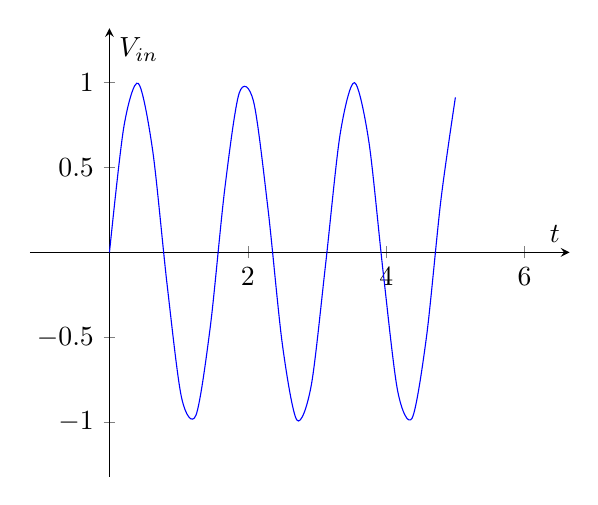
\begin{tikzpicture}
    \begin{axis}[
        domain=0:5,
        axis lines = middle,
        xmin = -0.5,
        xmax = 6,
        ymin = -1.1,
        ymax = 1.1,
        xlabel = $t$,
        ylabel = $V_{in}$,
        enlargelimits = true,
    ]
        \addplot[smooth,mark=none,color=blue] {sin(4*deg(x))};
    \end{axis}
\end{tikzpicture}
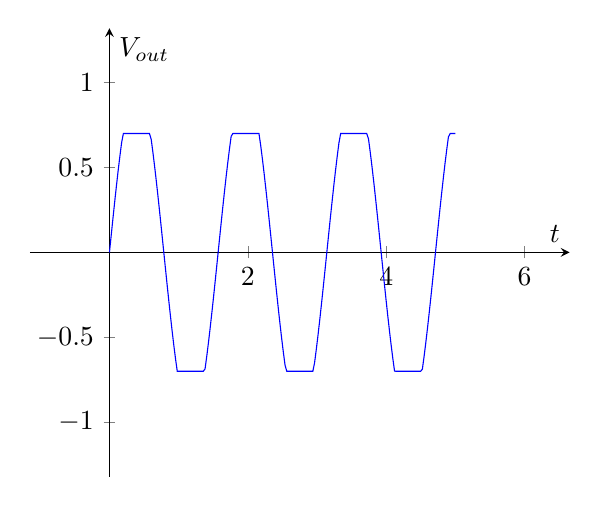
\begin{tikzpicture}
    \begin{axis}[
        domain=0:5,
        axis lines = middle,
        xmin = -0.5,
        xmax = 6,
        ymin = -1.1,
        ymax = 1.1,
        xlabel = $t$,
        ylabel = $V_{out}$,
        enlargelimits = true,
        y filter/.expression={y > 0.7 ? 0.7 : (y < -0.7 ? -0.7 : y)},
    ]
        \addplot[samples=200,mark=none,color=blue] {sin(4*deg(x))};
    \end{axis}
\end{tikzpicture}

  \caption{Impact of the diode limiter on the input sinusoidal voltage. Values that exceed the \SIrange{-0.7}{0.7}{V} range are clamped and the signal is distorted.}
  \label{fig:diode_limiter_signal}
\end{figure}


%%%%%%%%%%%%%%%%%%%%%%%%%%%%%%%%%%%%%%%%%%%%%%%%%%%%%%%%%%%%%%%%%%%%%%%%%%%%%%%%%%%%%%%
\subsection{First-Order Diode Clipper}
%%%%%%%%%%%%%%%%%%%%%%%%%%%%%%%%%%%%%%%%%%%%%%%%%%%%%%%%%%%%%%%%%%%%%%%%%%%%%%%%%%%%%%%
Combining the RC lowpass filter (\Figure{fig:rc_lowpass}) and the diode limiter (\Figure{fig:diode_limiter}) yields the first-order diode clipper (\Figure{fig:diode_clipper_circuit}). It is called "first-order" because only a single capacitor is used \cite{Parker2019}. If the input voltage is within the limiter's operational range, the circuit acts as a lowpass filter. If the voltage exceeds this range, it is clipped at the output and distortion is introduced.

The first-order diode clipper can be described by a nonlinear \ac{ODE} \cite{Yeh2007}
\begin{equation}
  \frac{\mathrm{d} V_\text{out}}{\mathrm{d}t} = \frac{V_\text{in} - V_\text{out}}{RC} - 2 \frac{I_\text{s}}{C} \sinh \left(\frac{V_\text{out}}{V_\text{t}}\right),
  \label{eq:diode_clipper_equation}
\end{equation}
where $V_\text{in}$ is the input voltage, $V_\text{out}$ is the output voltage, $t$ denotes time, $R$ is the serial resistance, $C$ is the parallel capacity, $I_\text{s}$ is the reverse saturation current, and $V_\text{t}$ is the thermal voltage. The last two are parameters of the diodes that can be measured \cite{Yeh2007}.

The parameter values of discrete elements used in the experiments were taken from \cite{Yeh2008}. They are summarized in \Table{tab:diode_clipper_element_parameters}.

\begin{table}
  \centering
  \caption{Parameter values of the discrete elements used in the diode clipper circuit. Source: \cite{Yeh2008}.}
  \begin{tabular}{c|c}
    \toprule
    \textbf{Parameter} & \textbf{Value} \\
    \midrule
    $R$ & \SI{2.2}{k\ohm} \\
    $C$ & \SI{10}{nF} \\
    $I_\text{s}$ & \SI{2.52}{nA} \\
    $V_\text{t}$ & \SI{45.3}{mV} \\
    \hline
  \end{tabular}
  \label{tab:diode_clipper_element_parameters}
\end{table}

$V_\text{in}$ is typically on the order of volts.

%%%%%%%%%%%%%%%%%%%%%%%%%%%%%%%%%%%%%%%%%%%%%%%%%%%%%%%%%%%%%%%%%%%%%%%%%%%%%%%%%%%%%%%
\subsection{Relation to Other Work}
%%%%%%%%%%%%%%%%%%%%%%%%%%%%%%%%%%%%%%%%%%%%%%%%%%%%%%%%%%%%%%%%%%%%%%%%%%%%%%%%%%%%%%%

The first-order diode clipper is a system particularly interesting in the context of ODENet, because it is governed by a known \ac{ODE} \cite{Yeh2007,Yeh2008}. Additionally, it was already modeled using a \ac{ResNet}-like architecture in \cite{Parker2019}. Thus, learning to imitate the diode clipper allowed the validation of ODENet and comparison to 
\begin{itemize}
    \item an \ac{LSTM}-based architecture from \cite{Wrightetal2020},
    \item a \ac{ResNet}-like architecture from \cite{Parker2019}, and
    \item a numerical solution using the \ac{ODE} from \cite{Yeh2007,Yeh2008}.
\end{itemize}

  \caption{Diode clipper circuit.}
  \label{fig:diode_clipper_circuit}
\end{figure}

The first-order diode clipper is a circuit frequently used to achieve signal distortion, e.\ g. in guitar amplifiers. Its schematic is shown on \Figure{fig:diode_clipper_circuit}. It can be regarded as consisting of two parts: an RC lowpass filter and a diode limiter.

%%%%%%%%%%%%%%%%%%%%%%%%%%%%%%%%%%%%%%%%%%%%%%%%%%%%%%%%%%%%%%%%%%%%%%%%%%%%%%%%%%%%%%%
\subsubsection*{RC Lowpass Filter}
%%%%%%%%%%%%%%%%%%%%%%%%%%%%%%%%%%%%%%%%%%%%%%%%%%%%%%%%%%%%%%%%%%%%%%%%%%%%%%%%%%%%%%%

\begin{figure}
  \centering
  \begin{tikzpicture}
%--------start graphics code --------
% \draw[step=0.5,very thin, black!20] (-1,-0.5) grid (6,2.5);
\path (0,0) coordinate (ref_gnd);
\draw
  (ref_gnd)++(0,2) node[ocirc] {}
  node[xshift=-2mm,yshift=4mm] {$V_{in}$}
  to [R=\(R\)] ++(2,0) node[circ] {}
  to ++(1,0)  node[ocirc] {}
  node[yshift=4mm] {$V_{out}$}
  ++(-1,0)
  to [C=\(C\)] ++(0,-2)
  node[ground] {};
%--------end graphics code ----------
\end{tikzpicture}

  \caption{RC lowpass filter.}
  \label{fig:rc_lowpass}
\end{figure}

The first part of the diode clipper circuit is an RC lowpass filter. An RC lowpass filter is shown in \Figure{fig:rc_lowpass}. The input-output voltage relation is governed by the following equation
\begin{equation}
  V_{out} = \frac{X_C}{\sqrt{R^2 + X_C^2}} V_{in},
  \label{eq:rc_circuit}
\end{equation}
where $V_{in}$ is the input voltage, $V_{out}$ is the output voltage, $X_C=\frac{1}{2\pi f C}$ is the capacitive reactance of the capacitor in the circuit, $C$ is its capacitance, $R$ is the resistor's resistance, and $f$ denotes the frequency of the input \ac{AC}.

The capacitor impedes low frequencies more; the lower the frequency, the higher the capacitive reactance. More capacitive reactance means larger voltage drop on the capacitor. Thus, assuming a constant magnitude across all frequencies of the input voltage, the output voltage is higher for low frequencies and the circuit behaves like a lowpass filter.

%%%%%%%%%%%%%%%%%%%%%%%%%%%%%%%%%%%%%%%%%%%%%%%%%%%%%%%%%%%%%%%%%%%%%%%%%%%%%%%%%%%%%%%
\subsection*{Diode Limiter}
%%%%%%%%%%%%%%%%%%%%%%%%%%%%%%%%%%%%%%%%%%%%%%%%%%%%%%%%%%%%%%%%%%%%%%%%%%%%%%%%%%%%%%%
\begin{figure}
  \centering
  \begin{tikzpicture}
%--------start graphics code --------
% \draw[step=0.5,very thin, black!20] (-1,-0.5) grid (6,2.5);
\path (0,0) coordinate (ref_gnd);
\draw
  (ref_gnd)++(0,2) node[ocirc] {}
  node[xshift=-2mm,yshift=4mm] {$V_{in}$}
  to [R=\(R\)] ++(2,0) node[circ] {}
  to ++(2,0)  node[circ] {}
  to ++(1,0)  node[ocirc] {} {}
  node[yshift=4mm] {$V_{out}$}
  ++(-1,0)
  to [D] ++(0,-2)
  to ++(-1,0)
  node[ground] {}
  to ++(-1,0)
  to [D] ++(0,2);
%--------end graphics code ----------
\end{tikzpicture}

  \caption{Diode limiter circuit.}
  \label{fig:diode_limiter}
\end{figure}

The second part of the diode clipper is the diode limiter also called a \emph{diode clamp} \cite{Malvino2016}. Its circuit is shown in the \Figure{fig:diode_limiter}. It consists of two inversely polarized diodes and a series resistor. This circuit could be further divided into a \emph{positive clipper} (by removing the diode on the left) and a \emph{negative clipper} (by removing the diode on the right). These names refer to which part of the input \ac{AC} signal (the positive or the negative) will be removed at the output.

If the diodes were ideal, i.\ e., they would behave as an open for voltages across smaller than 0 and as a short for voltages across larger than 0, $V_{out}$ would always be 0. However, to a second approximation, there diodes cause a voltage drop of \SI{0.7}{V} when conducting. Thus, the voltage cannot exceed the \SIrange{-0.7}{0.7}{V} range, being clamped when attempting to do so. The positive clipper guards the upper limit and the negative clipper guards the lower limit. The effect of passing an \ac{AC} signal through the diode limiter is shown in \Figure{fig:diode_limiter_signal}.

\begin{figure}
  \centering
  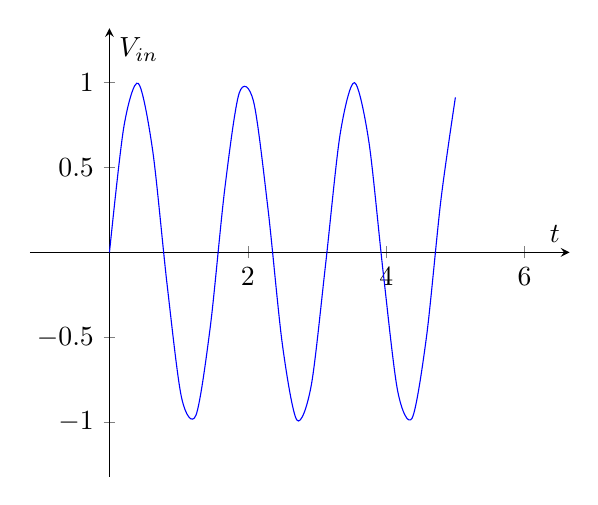
\begin{tikzpicture}
    \begin{axis}[
        domain=0:5,
        axis lines = middle,
        xmin = -0.5,
        xmax = 6,
        ymin = -1.1,
        ymax = 1.1,
        xlabel = $t$,
        ylabel = $V_{in}$,
        enlargelimits = true,
    ]
        \addplot[smooth,mark=none,color=blue] {sin(4*deg(x))};
    \end{axis}
\end{tikzpicture}
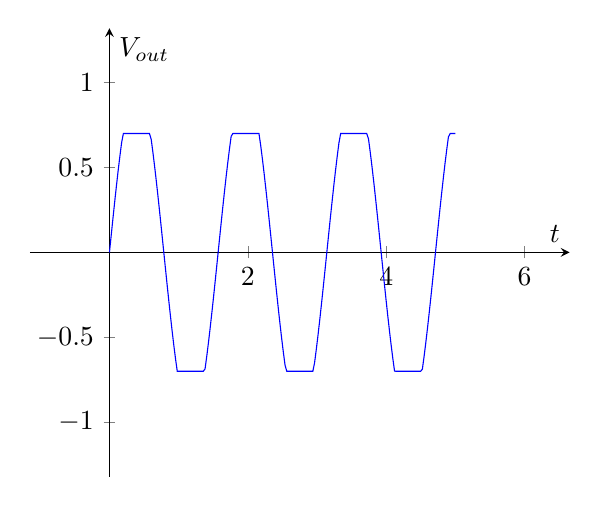
\begin{tikzpicture}
    \begin{axis}[
        domain=0:5,
        axis lines = middle,
        xmin = -0.5,
        xmax = 6,
        ymin = -1.1,
        ymax = 1.1,
        xlabel = $t$,
        ylabel = $V_{out}$,
        enlargelimits = true,
        y filter/.expression={y > 0.7 ? 0.7 : (y < -0.7 ? -0.7 : y)},
    ]
        \addplot[samples=200,mark=none,color=blue] {sin(4*deg(x))};
    \end{axis}
\end{tikzpicture}

  \caption{Diode limiter impact on the input sinusoidal voltage. Values that exceed the \SIrange{-0.7}{0.7}{V} range are clamped.}
  \label{fig:diode_limiter_signal}
\end{figure}


%%%%%%%%%%%%%%%%%%%%%%%%%%%%%%%%%%%%%%%%%%%%%%%%%%%%%%%%%%%%%%%%%%%%%%%%%%%%%%%%%%%%%%%
\subsubsection*{First-Order Diode Clipper}
%%%%%%%%%%%%%%%%%%%%%%%%%%%%%%%%%%%%%%%%%%%%%%%%%%%%%%%%%%%%%%%%%%%%%%%%%%%%%%%%%%%%%%%
Combining the RC lowpass filter (\Figure{fig:rc_lowpass}) and the diode limiter (\Figure{fig:diode_limiter}) yields the first-order diode clipper (\Figure{fig:diode_clipper}). It is called "first-order" because only a single capacitor is used \cite{Parker2019}. If the input voltage is within the limiter's operational range, the circuit acts as a lowpass filter. If the voltage exceeds this range, it is clipped at the output and distortion is introduced.

The first-order diode clipper can be described by a nonlinear \ac{ODE} \cite{Yeh2007}
\begin{equation}
  \frac{\mathrm{d} V_{out}}{\mathrm{d}t} = \frac{V_{in} - V_{out}}{RC} - 2 \frac{I_s}{C} \sinh \left(\frac{V_{out}}{V_t}\right),
\end{equation}
where $V_{in}$ is the input voltage, $V_{out}$ is the output voltage, $t$ denotes time, $R$ is serial resistance, $C$ is the parallel capacity, $I_s$ is the reverse saturation current, and $V_t$ is the thermal voltage. The last two are parameters of the diodes and can be extracted from measurement \cite{Yeh2007}. 

%%%%%%%%%%%%%%%%%%%%%%%%%%%%%%%%%%%%%%%%%%%%%%%%%%%%%%%%%%%%%%%%%%%%%%%%%%%%%%%%%%%%%%%

The first-order diode clipper is a system particularly interesting in the context of the ODENet, because it is governed by a known \ac{ODE} \cite{Yeh2007,Yeh2008}. Additionally, it was already modeled using a \ac{ResNet} type of architecture in \cite{Parker2019}. Thus, learning to imitate the diode clipper allowed for validation of the ODENet and comparison to 
\begin{itemize}
  \item an \ac{LSTM} architecture from \cite{Wrightetal2020},
  \item a \ac{ResNet}-like architecture from \cite{Parker2019}, and
  \item a numerical solution using the \ac{ODE} from \cite{Yeh2007,Yeh2008}.
\end{itemize}


%%%%%%%%%%%%%%%%%%%%%%%%%%%%%%%%%%%%%%%%%%%%%%%%%%%%%%%%%%%%%%%%%%%%%%%%%%%%%%%%%%%%%%%
\subsection{Phaser}
\label{subsec:phaser_intro}
%%%%%%%%%%%%%%%%%%%%%%%%%%%%%%%%%%%%%%%%%%%%%%%%%%%%%%%%%%%%%%%%%%%%%%%%%%%%%%%%%%%%%%%
%TODO add a figure of the phaser
Phaser is a filter-based, time-varying effect \cite{Zoelzer2011}. It applies a series of notches to the spectrum of the input signal. The center frequencies of these notches are controlled by a \ac{LFO} and constantly vary with respect to one another, each moving up and down the frequency range. Phaser is typically implemented by summing the input signal processed by a series of notch or allpass filters with a direct path \cite{Zoelzer2011}. Additionally, a feedback connection can be added around the filter chain \cite{Kiiski2016}. The feedback connection makes the phaser behavior more complex by introducing resonances and non-notch frequency boosting.

%%%%%%%%%%%%%%%%%%%%%%%%%%%%%%%%%%%%%%%%%%%%%%%%%%%%%%%%%%%%%%%%%%%%%%%%%%%%%%%%%%%%%%%
\section{Relation to Other Work}
\label{sec:relation_to_other_work}
%%%%%%%%%%%%%%%%%%%%%%%%%%%%%%%%%%%%%%%%%%%%%%%%%%%%%%%%%%%%%%%%%%%%%%%%%%%%%%%%%%%%%%%
The aim of this work is to investigate the applicability of the ODENet architecture to \ac{VA} modeling of audio effects. In comparison to dynamical systems examined in \cite{Karlsson2019}, networks modeling audio effects need to account for the input signal, which is not only time-varying but also time-discretized with a specific sampling rate. 

\cite{Parker2019} use an \ac{MLP} to learn the residual of a state-space system. The learned mapping steers the model through the state space of the device under study. The model is named \ac{STN}. Just as the original \ac{ResNet} paper \cite{He2015}, the residual not the derivative is learned, which is equivalent to the Euler method of solving \acp{ODE}. \cite{Parker2019} successfully applies \ac{STN} to model analog clipper circuits and an analog filter.

For modeling a phaser pedal, following \cite{Wright2020}, this work estimates the \ac{LFO} signal and uses it for conditioning the network. Therefore, it falls under the category of grey-box models. However, to achieve this goal, it uses a significantly different network architecture than \cite{Wright2020}.

